\TUchapter{Background}
\TUsection{Introduction}
This chapter provides background and context for the concepts, models, 
and examples involved in this thesis, including some insofar unpublished work
that does not necessarily comprise a contribution of this thesis. 

First, hybrid systems
and their newer counterparts, cyber-physical systems, are addressed. Existing
modeling frameworks for hybrid systems, particularly hybrid automata, are
defined, and an introduction to attack graphs is provided along with a
survey of their areas of research.

Next, section 2.4 presents at length the version of the attack graph model 
developed at the University of Tulsa and the components thereof. 
Finally, section 2.5 introduces the specific
domains of the two examples used throughout this thesis.
\TUsection{Cyber Physical Systems}
\TUsubsection{Hybrid Systems}
A system with both continuous (frequently physical) components and discrete (frequently digital)
components is said to be a \emph{hybrid system}, named for its characteristic blending of the
two domains. Examples abound in industrial controls,
although hybrid systems may also be fully physical (e.g., a bouncing ball that experiences continuous
behavior when rising and falling and discrete behavior when colliding with a surface).

The term hybrid system is an older one that was coined as researchers began to study the newly
pervasive reactive systems that arose as programmed control of the physical world became 
widespread ~\cite{alur1993hybrid}. It does not suffice to describe precisely
the types of systems with which this work is concerned: the subset of hybrid
systems that incorporate significant computer and networking components.

Nevertheless, the modeling of hybrid systems is well studied and provides a sufficient body
of relevant work from which to draw to warrant its inclusion. This chapter includes
background on a particularly relevant modeling framework for hybrid systems called the
hybrid automaton, which is used in this thesis as the standard benchmark against which to
compare hybrid modeling techniques.
\TUsubsection{Definition}
A newer term for the systems investigated in this thesis is \emph{cyber physical systems}
 (CPS).
Simply, a cyber physical system is a networked hybrid system: that is, a 
networked computer system that is tightly coupled to the physical world.
\TUsubsection{Challenges}
According to the 2008 Report of the Cyber-Physical Systems Summit, ``The principal barrier to 
developing CPS is the lack of a theory that comprehends cyber and physical resources in a 
single unified framework.''~\cite{summitreport2008}

The summit further identified as part of the necessary scientific and technological foundations of
cyber physical systems both (1) new modeling frameworks that ``explicitly address new observables'' and (2)
studies of privacy, trust, and security including ``theories of cyber-physical inter-dependence''~\cite{summitreport2008},
a major theme of this work.

Crenshaw and Beyer recently enumerated four principal challenges in 
cyber-physical systems:
their concentration in safety critical domains, their integration of 
unrelated systems, their dependence upon unreliable 
data collection, and their pervasiveness~\cite{crenshaw2010upbot}.
\TUsubsection{Hybrid Automata}
\TUsubsubsection{Definition}
A valuable formalism for modeling hybrid systems in isolation and with limited 
interconnection is the hybrid automaton (HA) of Alur, \emph{et al.}~\cite{alur1993hybrid}. 
This section introduces the version of the formalism described in 1996 by 
Henzinger~\cite{henzinger1996theory}, to which a reader interested in more 
than a superficial understanding is referred. 

Formally,
a hybrid automaton $H$ is made up of a set $X$ of real-valued state variables, 
a set $\dot{X}$ of their first derivatives, a set of operational modes and 
guarded switches between the modes, and predicates describing continuous 
evolution over time.

One can think of a hybrid automaton as a pairing of a finite state 
machine---whose states (``modes'') and transitions (``switches'') denote the 
discrete-domain behavior of the system---with differential equations that
govern its continuous-domain behavior.

Modes may be decorated with \emph{invariant} conditions (when the 
system may be in that mode), \emph{flow} conditions (how the 
continuous state variables may evolve while in that mode), and \emph{initial}
conditions (when and if the automaton may start in that mode). 
Switches are decorated with 
\emph{jump} conditions, which determine
(1) when the switch is allowed to be taken, and (2) the discrete changes 
in state variables due to that
switch's activation.

A simple example of a hybrid automaton, given in Fig.~\ref{fig:thermostat}, 
is a
heater thermostat~\cite{henzinger1996theory}. The vertices in the automaton represent 
its operating modes, and the edges represent its control
switches. In the ``Off'' mode, the temperature (given by $x$) must be greater 
than or equal to 18, and
its first derivative with respect to time (denoted $\dot{x}$) is $-0.1x$, which 
represents a cooling of
the environment. When the temperature is strictly less than 19, the switch from
off to on is available (but
not mandatory until $x < 18$). The switch from on to off behaves similarly.

\begin{figure}
\centering
\begin{dot2tex}[options=-t raw --autosize]
digraph G {
    rankdir=LR;
    
    Off [texlbl="$\begin{matrix} \text{Off} \\ \
    \dot{x} = -0.1x \\ \
    x \geq 18 \\ \
    \end{matrix}$"];
    
    On [texlbl="$\begin{matrix} \text{On} \\ \
    \dot{x} = 5 - 0.1x \\ \
    x \leq 22 \\ \
    \end{matrix}$"];
        
    Off -> On [label=" " texlbl="$x < 19$"];
    
    On -> Off [label=" " texlbl="$x>21$"];
}
\end{dot2tex}
\caption{Thermostat hybrid automaton}
\label{fig:thermostat}
\end{figure}

\TUsubsubsection{Shortcomings}
A hybrid automaton is not guaranteed to
have a valid execution, and computing whether it does or not is 
non-trivial~\cite{lygeros1999existence}.
Model checking has been developed for only some subclasses of 
automata~\cite{henzinger1997hytech, frehse2005phaver}, and many useful
properties of them are undecidable~\cite{henzinger1998s}.

However, there are further issues when considering hybrid automata
for the study of cyber-physical systems. One of the hallmarks of cyber-physical systems is a
distributed and highly networked nature. While HAs provide a
natural model for the discrete-continuous boundary, they have only a rudimentary
notion of communication, and when used in large
topologies have significant scaling problems, both computationally and cognitively.
\TUsubsubsection{Alternatives}
Attempts have been made to improve the hybrid automaton's network modeling
capability. The designation of shared
actions and shared variables as ``input'' or ``output'' is a popular tactic, 
as in the powerful hybrid I/O 
automaton~\cite{lynch1996hybrid, lynch2001hybrid}, its descendant the
timed I/O automaton~\cite{kaynar2010theory}, and in the PHAVer model 
checker~\cite{frehse2005phaver}.

Similarly, the work of this thesis is partly an outgrowth of 
this strategy. An object example of that preliminary work's inherent issues
is given in Fig.~\ref{fig:linkmachine},
a considered ``hybrid link automaton'' prototype. This models a link between two
unpictured hybrid automata called $S$ (the message source) and $D$ (the message
destination). The link is named $\lambda$, and the message is denoted with 
$\mu$. The intent was that the automaton be parameterized, with many instances
of it and similar link machines be used in the model of a single system.
The link exhibits the following behaviors:

\begin{description}
\item[Messaging] The messages in the automaton are encoded as either
    ``source : link : message'' for a message incoming to the link from $S$, or
    ``link : destination : message'' for outgoing to $D$. These are actually 
    hybrid automata events, which are used with its composition facility to 
    model this messaging.
\item[Unreliable delivery] The unguarded switch from the transmit to idle mode
    permits transition back to idle without the actual emission of a message.
\item[Message injection] The unguarded switch from Idle to Transmit permits a
    message to transmit without being received.
\item[Latency] The clock ($C_{\lambda\mu}$, which increments at a rate 
    $\dot{C}_{\lambda\mu}$) permits a certain waiting period between entry to
    the Transmit mode and actual transmission of the message.
\item[Rudimentary mutual exclusion] The Wait mode permits only a single
    message to be on the wire at a time.
\end{description}

This strategy may have a place in modeling some systems but falls short of 
the goal of  modeling complex hybrid systems 
with more conventional computer networks---it is simply too low level.
\begin{figure}
\centering
\begin{dot2tex}[options=-t raw --autosize]
digraph G {
    rankdir=TD;
    idle [shape=circle, texlbl= \
    "$ \begin{matrix} \lambda : \mu : \text{Idle} \\ \
    \dot{C}_{\lambda \mu} = 0 \\ \
    C_{\lambda \mu} = 0 \end{matrix} $"];
    
    transmit [shape=circle, texlbl= \
    "$ \begin{matrix} \lambda : \mu : \text{Transmit} \\ \
    \dot{C}_{\lambda \mu} = 1 \\ \
    C_{\lambda \mu} < l \wedge w_{\lambda}=1  \end{matrix}$"];
    
    wait [shape=circle, texlbl= \
    "$\begin{matrix} \lambda : \mu : \text{Wait} \\ \
    w_{\lambda}=1 \\ \
    \end{matrix}$"];
    
    transmit -> idle [label= " " \
    texlbl="$\begin{matrix} \lambda : D : \mu \\ \
    C_{\lambda \mu} < l \\ \
    C_{\lambda \mu} := 0 \wedge w_{\lambda}:=0 \
    \end{matrix}$"];
    
    idle -> transmit [label= " ", \
    texlbl= "$\begin{matrix} S : \lambda : \mu \\ \
    w_{\lambda}=0 \\ \
    w_{\lambda}:=1 \\ \
    \end{matrix}$"];
    
    idle -> wait [label= " ", \
    texlbl= "$\begin{matrix} S : \lambda : \mu \\ \
    w_{\lambda}=1 \\ \
    \end{matrix}$"];
    
    wait -> transmit [label= " ", \
    texlbl= "$\begin{matrix} \
    w_{\lambda}=0 \\ \
    w_{\lambda}:=1 \\ \
    \end{matrix}$"];
    
    wait -> wait [label= " ", \
    texlbl= "$\begin{matrix} S : \lambda : \mu \\ \
    \end{matrix}$"];
    
    idle -> idle [label= " ", \
    texlbl="$\lambda : D : \mu$"];
    
    idle -> transmit;
    
    transmit -> idle;
    idle -> idle [label= " ", \
    texlbl="$S : \lambda : \mu$"];
    
}
\end{dot2tex}
\caption{Example hybrid link automaton}
\label{fig:linkmachine}
\end{figure}

Although the hybrid automaton is the gold standard for modeling hybrid systems, 
other frameworks do exist such as hybrid process 
algebras~\cite{cuijpers2005hybrid, bergstra2005process},
entirely symbolic systems with many of the same properties and drawbacks as
hybrid automata. Hybrid Petri nets are similar to hybrid automata in that they
pair a standard discrete model (in this case, Petri nets instead of finite state
automata) with differential equations to model the continuous side of the
system or process~\cite{champagnat1998petri}.
\TUsection{Attack Trees and Graphs}
\TUsubsection{Introduction}
An attack graph is one of several related formalisms that utilize graph theory to
model the state space of computer systems attacks with interacting elements. 
Perhaps they are best introduced
when presented as an alternative to a similar model called an attack tree.
\TUsubsection{Attack Trees}
An attack tree is a goal-oriented model of an abuse of a system~\cite{schneier1999modeling}.
The root of the tree represents the attacker's goal, and the children of any given node represent
its prerequisites. For example, consider the goal of
stealing a car, which is modeled in a simple attack tree in Fig.~\ref{fig:attacktree}.

The attacker must start the car and drive away; this could be accomplished either by breaking
in and hot wiring the car, or by stealing the owner's key and using it to subsequently steal the
car. The root of the tree represents the final goal of the theft, with prerequisite goals
flowing upward from the leaf nodes.
\begin{figure}
\centering
\begin{dot2tex}[options=-t raw --autosize]
digraph G {
    rankdir=BU;
    StealCar [texlbl="Steal car" shape=rectangle];
    UseKey [texlbl="Start car with key" shape=rectangle];
	HotWire [texlbl="Hotwire car" shape=rectangle];
	StealKey [texlbl="Steal owner's key" shape=rectangle];
	OpenDoor [texlbl="Access car interior" shape=rectangle];
	CallLocksmith [texlbl="\begin{tabular}{c}Impersonate owner \\to locksmith\end{tabular}" shape=rectangle];
	BreakWindow [texlbl="\begin{tabular}{c}Break in \\through window\end{tabular}" shape=rectangle];
	UseKey -> StealCar;
	HotWire -> StealCar;
	StealKey -> UseKey;
	OpenDoor -> HotWire;
	CallLocksmith -> OpenDoor;
	BreakWindow -> OpenDoor;
}
\end{dot2tex}
\caption{Simple car theft attack tree}
\label{fig:attacktree}
\end{figure}

Attack trees are goal oriented:
the consequences of the attack are known, and the generation process is the 
enumeration of the means by which those consequences could be reached. 
It is, as an attack model, agnostic to the
underlying system. This makes it difficult to generate automatically. Finally, and perhaps
most significantly, it captures the ways in which an attacker's actions interact and 
depend upon each other.

This approach is not necessarily the most useful for system stakeholders. It
requires that one work backward from the attack to the system state
necessary to realize the attack. If, instead, an analyst desires to work from a system characterization
and explore the attack space permitted by that system characterization, the attack tree framework
must be in some sense turned upside down. 
Attack graphs do exactly that.
\TUsubsection{Attack Graphs}
\TUsubsubsection{Introduction}
In contrast to attack trees, attack graphs permit a topology-aware exploration
of the state space of a system. They engage a graph theoretic model in which 
vertices represent individual system states, and edges represent state 
transitions caused by an adversary. The concept as originally introduced 
shares with all modern incarnations notions of attack patterns to be bound to state 
transitions; network elements and their individual configurations; and network 
topology. Also originally present but rarer in modern versions are
representations of the attacker's capabilities and edge weights representing 
likelihood~\cite{phillips1998graph}. A similar structure called a privilege 
graph was introduced around the same time~\cite{dacier1994privilege}.

Most approaches to attack graph modeling represent exploits (attack patterns) using
preconditions and postconditions~\cite{lippmann2005annotated, 
templeton2001requires}. Exploits are chained together by matching preconditions
in a state node's underlying system model and applying their postconditions to 
generate a successor state.
\TUsubsubsection{Model Types}
The modeling substrates of stateful attack graphs can be broadly separated into 
two schools of thought, separated by the philosophy that guides the representation of the underlying
network model over which network states and transitions are computed.

Specification of the underlying network model may be done with only very loose
restrictions, allowing arbitrary keywords as named qualities and topologies of 
network objects, as is favored for example in the work of George Mason 
University~\cite{ammann2002scalable, wang2006minimum}.
This thesis employs this method, permitting more straightforward adaptation 
into the continuous domain.

The alternative is domain-driven, confining the modeler to
terms that impose explicit computer networking 
concepts onto the model~\cite{templeton2001requires}.
This permits generation and analysis to take a
more nuanced view of a network state, including reachability analysis to determine whether a
given topology permits communication between two hosts~\cite{ingols2009modeling}.

Another variant of the attack graph, representing a fairly significant departure
from the original formalism, is the exploit dependency graph (or attack
dependency graph), which encodes similar information in a graph of conditions
and exploits, rather than of states~\cite{jajodia2005topological, 
noel2004managing, louthan2011toward}.

\TUsubsubsection{Research Directions}
Research in attack graphs is spread throughout a variety of pathways. These include
merely evaluating a network's security~\cite{ammann2002scalable}, specification of formal languages
to represent attack graphs~\cite{templeton2001requires}, intrusion detection system 
integration~\cite{tidwell2001modeling}, automatic generation of security recommendations~\cite{wang2006minimum},
and reachability analysis between hosts in a single network state~\cite{ingols2009modeling}. 
For a thorough literature review up to 2005 and more detailed discussion of popular research directions, 
refer to the work of Lippmann and Ingols~\cite{lippmann2005annotated}.

Attack graph work can be considered to fall into four broad categories, referenced
occasionally throughout this work by the following names.
\begin{description}
\item[Modeling] Attack graph modeling concerns the development of the underlying representation
	and use of that representation to model systems. Terminology belongs here, as do efforts to
	automatically generate network models from real networks and exploit patterns from vulnerability
	databases.
\item[Generation] Attack graph generation is the process of building a graph out of a model by
	closing the state space over its exploits. This is where most performance work is concentrated.
	The work that enables a representation of time is shared between generation
    and modeling. Constraints (such as monotonicity) on the progression of 
    state transitions also fall under the generation category.
\item[Analysis] Analysis of attack graphs draws conclusions from attack graphs.
    Work here includes integration with intrusion detection
	systems, automatic delivery of mitigation recommendations, and the 
    identification of states' security consequences.
\item[Visualization] Visualization of attack graphs seeks to reduce or eliminate their
	known cognitive scalability issues; the goal is to deliver the results of the other three
	steps in a meaningful fashion.
\end{description}

This thesis is mainly concerned with the modeling stage. Some amount of work
is included in the generation stage, particularly
dealing with the progression of time.



%%%%%%%%%%%%%%%%%%

\TUsection{Attack Graph Generation and Modeling}
This section presents a version of the attack graph modeling framework specific
to traditional information systems. The framework has a very permissive 
modeling language that
includes notions of assets, qualities, topologies. Assets represent potentially
attackable system components; qualities assign an arbitrary string value to a named
property of an asset, and topologies connect pairs of assets.
Exploit patterns have preconditions and postconditions on parameterized assets
that can be bound at generation time to assets to create state transitions.
\TUsubsection{Intuitive Definition}
An attack graph is comprised of the following components.
\begin{description}
	\item[Assets] Assets are the security principals in the attack graph 
        formalism. For example, an asset may represent a host, an attacker, or 
        a document. Assets are specified with unique names, and they are 
        decorated with \emph{qualities} and \emph{topologies}.
	\item[Qualities] Qualities represent properties of an asset, such as a software package or
		version, or whether it is offline, online, or in sleep mode. 
        Qualities are key/value pairs, where both the key and the value are 
        strings.
	\item[Topologies] Topologies represent relationships between two assets.
        In addition to network connections, these include abstract 
        relationships such as trust or access. Topologies are directed and
		named with strings. Together with qualities, topologies make up the
		network state's collection of facts, also called the ``fact base''.
	\item[State] A network or system state is comprised of all of the facts about the system's asset
		collection. A network model's state is fully described by the asset collection and the fact base;
		given the constant asset collection, a state is uniquely described by its fact base. The fact
		base is all the qualities and topologies that are valid for that state.
	\item[Exploit patterns] Exploit patterns are general templates for how the 
        actions of the attacker can alter the system state by inserting and 
        removing qualities and topologies (but not assets).
		They are written as functions that take parameters corresponding to assets,
        are guarded by preconditions, and specify a set of postconditions:
		insert and delete actions on qualities and topologies to update the 
        fact base and therefore generate new network states.
\end{description}
\TUsubsection{Formal Definition}
\label{sec:domains}
\TUsubsubsection{Primitive Domains}
To clarify the attack graph formalism,
this section provides a more formal definition of its components' domains.
The primitive domains describe the atomic units of
the formalism: assets, properties (qualities), values (qualities), relationships (topologies),
vulnerabilities (exploit pattern identifiers), parameters (free asset variables in the attack
patterns), and operations (used in postconditions representing insert or delete actions).
See Fig.~\ref{fig:primitivedomains} for these elements' formal notation.

\begin{figure}
\begin{align*}
    \mathcal{A} :& \text{assets} \\
    \mathcal{P} :& \text{properties (quality names)} \\
    \mathcal{V} :& \text{values (property values)} \\
    \mathcal{R} :& \text{relationships (topology names)} \\
    \mathcal{W} :& \text{vulnerabilities (exploit pattern names)} \\
    \mathcal{I} :& \text{parameters (free asset names)} \\
    \text{Op} =& \left\{\text{ins}, \text{del} \right\}
\end{align*}
\caption{Attack graph primitive domains}
\label{fig:primitivedomains}
\end{figure}

\TUsubsubsection{Compound Domains}
Compound domains are composed of combinations
of members of the primitive domains. These form the level of abstraction that it is
most convenient to discuss intuitively.
\begin{description}
    \item[Qualities] Qualities bind an asset to a property to a value; therefore their
        domain is their Cartesian product. The $n$ subscripts denote that
        these are bound qualities of a network state, rather than free qualities in
        exploit preconditions and postconditions:
        \begin{align*}
            \mathcal{Q}_n &: \mathcal{A} \times \mathcal{P} \times \mathcal{V}
        \end{align*}
    \item[Topologies] Topologies bind an asset to another asset through a relationship; therefore their
        domain is the Cartesian product of those domains:
        \begin{align*}
            \mathcal{T}_n&: \mathcal{A} \times \mathcal{A} \times \mathcal{R}
        \end{align*}
    \item[Network states] A network state is a collection of assets, and a fact base
        of qualities and topologies; the domain of a network state is the Cartesian product
        of the power sets of these domains:
        \begin{align*}
            \mathcal{N}&: \mathbb{P}(\mathcal{A}) \times \mathbb{P}(\mathcal{Q}_n) \times \mathbb{P}(\mathcal{T}_n)
        \end{align*}
    \item[Exploit patterns] Exploit patterns, taken from the domain $\mathcal{E}$,
		depend upon free versions of qualities and topologies,
		members of $\mathcal{I}$ rather than $\mathcal{A}$. These are used in
		preconditions and, with operators, postconditions:
        \begin{align*}
			\mathcal{Q}_e&: \mathcal{I} \times \mathcal{P} \times \mathcal{V} \\
			\mathcal{T}_e&: \mathcal{I} \times \mathcal{I} \times \mathcal{R} \\
			\text{Preconditions } \mathcal{P}rc_e &: \mathbb{P}(\mathcal{Q}_e) \times \mathbb{P}(\mathcal{T}_e) \\
			\text{Postconditions } \mathcal{P}oc_e&: \mathbb{P}((Op,\mathcal{Q}_e)) \times \mathbb{P}((Op,\mathcal{T}_e)) \\
			\mathcal{E}&: \mathcal{W} \times \vec{\mathcal{I}} \times  \mathcal{P}rc \times \mathcal{P}oc
        \end{align*}
    \item[Attacks] An exploit pattern whose parameters have been bound to assets is referred to as an
		attack. It takes a similar appearance:
		\begin{align*}
			\text{Preconditions } \mathcal{P}rc_n &: \mathbb{P}(\mathcal{Q}_n) \times \mathbb{P}(\mathcal{T}_n) \\
			\text{Postconditions } \mathcal{P}oc_n&: \mathbb{P}((Op,\mathcal{Q}_n)) \times \mathbb{P}((Op,\mathcal{T}_n)) \\
			\mathcal{X}&: \mathcal{W} \times \vec{\mathcal{I}} \times  \mathcal{P}rc \times \mathcal{P}oc
        \end{align*}
\end{description}

\TUsubsection{Specification Language}
The attack graph generator does 
not use this formal notation to represent system elements, instead favoring a 
more user friendly specification language. 

\TUsubsubsection{Network Model Specification}
The first component of the specification itself is an asset list. Following the
asset list, the initial
fact base is specified as a semicolon separated list of qualities and 
topologies. An example network model specification is found in 
Fig.~\ref{fig:nmspec}.

\begin{figure}
\begin{lstlisting}
network model = 
    assets :
    asset_1;
    asset_2;
    asset_3;

facts :
	quality:asset_1,quality_1,value_1;
	quality:asset_2,quality_1,value_2;
	topology:asset_1,asset_2,topology_1;
	topology:asset_2,asset_3,topology_2;
    topology:asset_3,asset_2,topology_2;
.
\end{lstlisting}
\caption{Example background network model specification}
\label{fig:nmspec}
\end{figure}
\TUsubsection{Exploit Specification}
Exploit patterns resemble functions whose bodies are lists of preconditions,
which are identical in form to the facts in the network model (except that their
assets are free rather than bound) and postconditions, which are simply
deletions or insertions (with overwrite semantics) of facts. An example may be 
found in Fig.~\ref{fig:xpspec}.

\begin{figure}
\begin{lstlisting}
exploit exploit_1(asset_param_1,asset_param_2)=
    preconditions:
        quality:asset_param_1,quality_1,value_1;
        topology:asset_param_1,asset_param_2,topology_1;
    postconditions:
        delete topology:asset_param_1,asset_param_2,topology_1;
        insert quality:asset_param_1,quality_1,value_2;
.
\end{lstlisting}
\caption{Example background exploit pattern specification}
\label{fig:xpspec}
\end{figure}

\TUsubsection{Generation Process}
Attack graph generation is the process of chaining exploits to enumerate the
attack space~\cite{campbell2002modeling,phillips1998graph,sheyner2002automated}.
Modern methods for generating attack graphs
share a common general architecture,
pictured in Fig. \ref{fig:generation}. The attack graph generation
process combines network state and exploit patterns as input, applying exploit 
postconditions back onto the network state to generate its output of successor 
states.

\begin{figure}
\centering
\begin{dot2tex}[options=-t raw --autosize]
digraph G {
    Generator [texlbl="Generation Engine", shape="rectangle"];
    Exploits [texlbl="\begin{tabular}{c}Exploit Rules\\ (Generic transitions)\end{tabular}", shape="ellipse"];
	State [texlbl="\begin{tabular}{c}Network State\\ (Facts)\end{tabular}", shape="ellipse"];
	Exploits -> Generator [texlbl="\begin{tabular}{c}1a. Read exploit \\ preconditions\end{tabular}", label=" "];
	State -> Generator [texlbl="\begin{tabular}{c}1b. Match preconditions \\ with network state\end{tabular}", label=" "];
	Generator -> State [texlbl="\begin{tabular}{c}2. Apply new\\ network state\end{tabular}", label=" "];
}
\end{dot2tex}
\caption{Attack graph generation process}
\label{fig:generation}
\end{figure}

A maximum attack graph ``depth'' (really 
maximum permitted shortest path length from the
node representing the initial state) is selected before generation begins, and
no self loops are permitted, though loops in general are allowed.

As this work's specific algorithm is a contribution, it is given
more detailed treatment in chapter 3.

\TUsection{Case Studies}
Among the examples appearing in this work, two are based on specific real world
scenarios.
The first is an attack on a traditional information system, based upon an offensive educational exercise
deployed at the University of Tulsa. The second is the 
denial of service through battery exhaustion of a simple
cyber-physical system of active radio frequency identification (RFID) tags and readers.
\TUsubsection{Blunderdome}
\label{sec:blunderdome}
The first case study is an attack on a simulated educational network deployed as part of a
security engineering course. Dubbed the Blunderdome, it featured a firewalled network of
two hosts available per attacker. See Table \ref{table:blundertasks} for a listing of the stages and
their preconditions and results. The attacker was required to log into a server by cracking
its weak SSH key (due to an operating system vulnerability), execute an elevation of privilege (due
to a Linux kernel vulnerability), log into the web server, and execute a SQL injection attack to
change a simulated grade. The architecture from the exercise is provided in 
Fig.~\ref{fig:blunderarch}, published in~\cite{louthan2010blunderdome}.

\begin{figure}
\centering
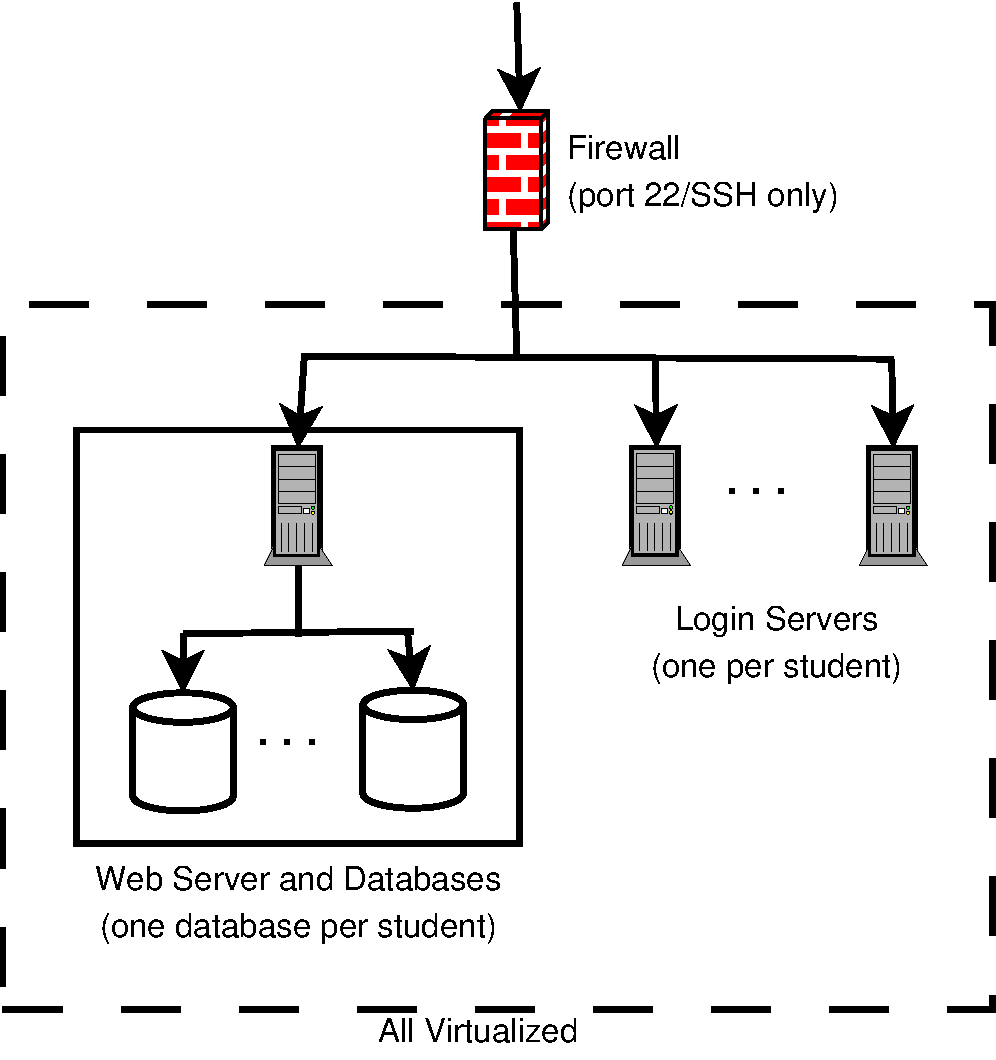
\includegraphics[width=3in]{blunderarch}
\caption{Blunderdome network architecture}
\label{fig:blunderarch}
\end{figure}

\begin{table}
\centering
\begin{tabular}{r|p{1.25in}|p{1.35in}|p{1.75in}}
Stage & Precondition	&	Attack	&	Postcondition \\ \hline \hline
1 & \raggedright Given weak SSH public key
	& \raggedright Find private key &  Login server user access \\ \hline
2 & \raggedright User-level access & \raggedright \texttt{vmsplice} privilege escalation 
	& Root on login server; web server credentials \\ \hline
3 & \raggedright Web application access & \raggedright SQL injection & Altered grade
\end{tabular}
\caption{Stages of the Blunderdome attack}
\label{table:blundertasks}
\end{table}
\TUsubsection{RFID Denial of Sleep}
\label{sec:bg:rfid}
The second case study is a denial of service attack
on the ISO 18000-7 RFID tag inventory system similar to those used by the United States
Department of Defense for freight tracking and the Department of Energy for tracking spent
fuel containers~\cite{chen2009radiofrequency}. The attack
is similar to the ones described by Buennemeyer, \emph{et al.}~\cite{buennemeyer2006battery},
and is of a newly distinguished class of attacks sometimes termed \emph{denial
of sleep attacks}~\cite{brownfield2005wireless}~\cite{raymond2009effects}.

These ISO 18000-7 RFID tags are active and battery powered; they are used for inventory and
shipment tracking. In particular, they are used by the Department of Energy to monitor
the location and seal status of
radioactive material containers, greatly reducing workers' radiation exposure. 
The batteries on the tags should last as long as
possible in order to limit radiation exposure to maintenance workers, and
the loss of power to these devices has safety consequences.
An energy draining attack to deplete the tags' batteries could significantly
speed this loss of power.

The ISO 18000-7 tags have two modes: an active mode, and a sleep mode in which their
power consumption is significantly reduced. The active mode has a 30 second timeout,
which causes them to sleep unless the timer is reset by a valid
command from the reader or a wake-up signal. In sleep mode, the tags can only
be awoken by a wake-up command.
A denial of sleep attack occurs when the tag is not permitted to enter sleep mode or is
awoken more frequently than normal.

This attack can be realized in two ways. The first is for a second, rogue 
RFID reader to be placed by the attacker within range of active tags. The
second is for the attacker to compromise an existing reader by hacking into a computer
system connected to it via a network.

Hybrid automata serve to represent the behavior of the devices themselves quite well.
Fig.~\ref{fig:readerha} represents the reader (legitimate or rogue), which does nothing but 
transmit commands and
wake-up signals, which can come at any time. Under
ordinary conditions this might take place over the course 
of several years before the batteries in the tags are 
drained~\cite{chen2009radiofrequency}.

\begin{figure}
\centering
\begin{dot2tex}[options=-t raw --autosize]
digraph G {
    rankdir=LR;
    idle [shape=circle, texlbl= "Reading"];    
	idle -> idle [label="Command"];
	idle -> idle [label="WakeUp"];
}
\end{dot2tex}
\caption{Hybrid automaton model of the RFID reader}
\label{fig:readerha}
\end{figure}

Fig.~\ref{fig:tagha} depicts a model of a tag.
It has two state variables: $c$, which represents the active mode timeout
clock, and $B$, which represents battery capacity. 
When active, the battery drains at the arbitrarily chosen rate of -50 
units per second. In sleep mode,
the battery drains at a rate of -1 per second. No restrictions are placed on the starting condition
of the battery. The two automata are composed using two shared 
actions: \emph{WakeUp} and \emph{Command}, which
synchronize the switches they decorate between the automata.

\begin{figure}
\centering
\begin{dot2tex}[options=-t raw --autosize]
digraph G {
    rankdir=TD;
    awake [shape=circle, texlbl= \
    "$ \begin{matrix} \text{Awake} \\ \
    \dot{c}_{\lambda \mu} = -1 \wedge \dot{B}=-50 \\ \
    c>0 \wedge B>0 \end{matrix} $"];
    
    asleep [shape=circle, texlbl= \
    "$ \begin{matrix} \text{Asleep} \\ \
    \dot{c} = 1 \wedge \dot{B} = -1 \\ \
    B>0  \end{matrix}$"];
    
    dead [shape=circle, texlbl= \
    "$ \begin{matrix} \text{Dead} \\ \
    \dot{c} = 0 \wedge \dot{B} = 0 \\ \
    B=0  \end{matrix}$"];
	
	init [shape=none, label=""];
	
	init -> awake [label= " " \
    texlbl="$\begin{matrix} c=30 \
    \end{matrix}$"];
	
    awake -> awake [label= " " \
    texlbl="$\begin{matrix} \text{Command} \\ \
    c := 30 \
    \end{matrix}$"];
	
	awake -> awake [label= " " \
    texlbl="$\begin{matrix} \text{WakeUp} \\ \
    c := 30 \
    \end{matrix}$"];
	
	awake -> asleep [label= " " \
    texlbl="$\begin{matrix} \text{Timeout} \\ \
	c=0 \
    \end{matrix}$"];
	
	awake -> dead [label= " " \
    texlbl="$\begin{matrix} \text{Die} \\ \
	B=0 \
    \end{matrix}$"];
	
	asleep -> asleep [label= " " \
    texlbl="$\begin{matrix} \text{Command} \
    \end{matrix}$"];
	
	asleep -> awake [label= " " \
    texlbl="$\begin{matrix} \text{WakeUp} \\ \
    c := 30 \
    \end{matrix}$"];
    
	asleep -> dead [label= " " \
    texlbl="$\begin{matrix} \text{Die} \\ \
	B=0 \
    \end{matrix}$"];
    
	dead -> dead [label= " " \
    texlbl="$\begin{matrix} \text{Command} \
    \end{matrix}$"];
	
	dead -> dead [label= " " \
    texlbl="$\begin{matrix} \text{WakeUp} \
    \end{matrix}$"];
	
}
\end{dot2tex}
\caption{Hybrid automaton model of the case study active RFID tags}
\label{fig:tagha}
\end{figure}